\model{Students and Teachers}

\begin{center}
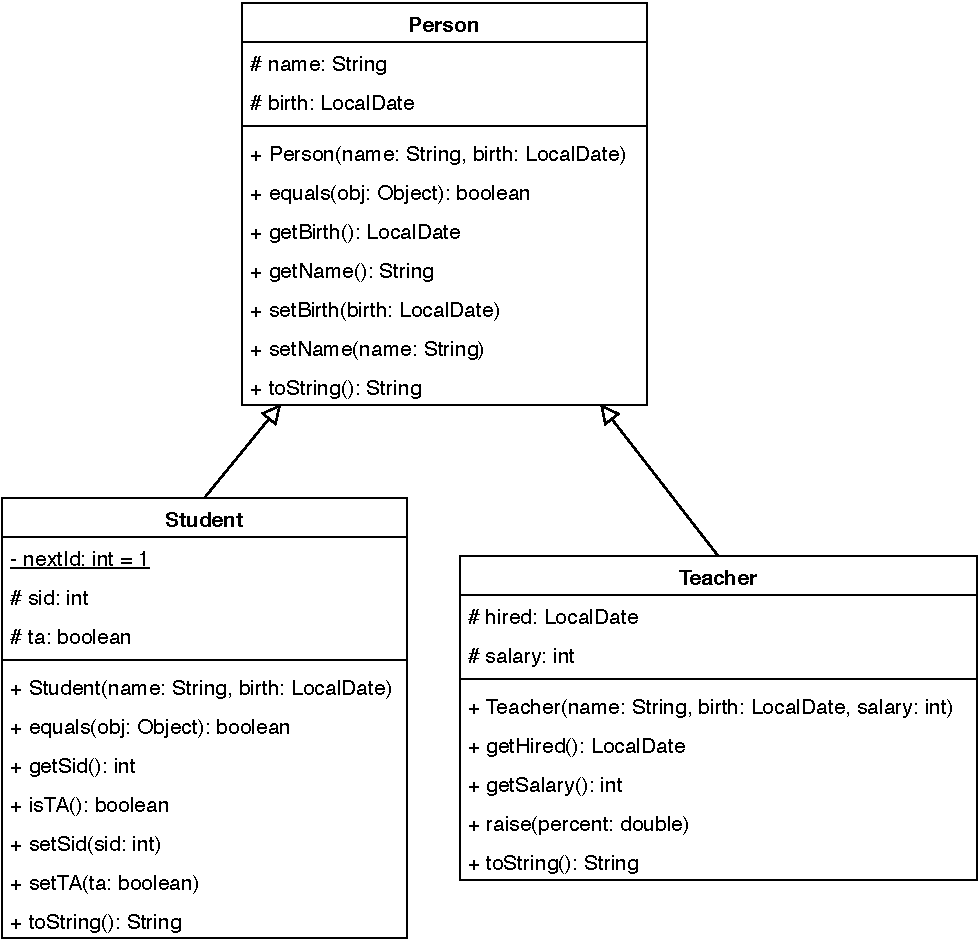
\includegraphics[scale=1]{PersonStudentTeacher.pdf}
\end{center}


\quest{15 min}


\Q Based on the UML diagram:

\begin{enumerate}
\item What attributes does a \java{Student} object have?
\ans{name, birth, sid, ta}

\item What attributes does a \java{Teacher} object have?
\ans{name, birth, hired, salary}

\item Which methods does \java{Student} override?
\ans{equals and toString}

\item Which methods does \java{Teacher} override?
\ans{toString}
\end{enumerate}


\Q Based on the UML diagram:

\setlength{\defaultwidth}{20em}

\begin{enumerate}
\item Which methods does a \java{Student} and a \java{Teacher} have in common? (i.e., inherited)
\begin{answer}[1em]
getBirth, getName, setBirth, setName
\end{answer}

\item Which methods does a \java{Student} object have that a \java{Teacher} object does not have?
\begin{answer}[1em]
getSid, isTA, setSid, setTA
\end{answer}

\item Which methods does a \java{Teacher} object have that a \java{Student} object does not have?
\begin{answer}[1em]
getHired, getSalary, raise
\end{answer}
\end{enumerate}

\vspace{-2em}


\Q Fill in each blank with either ``is a'' or ``has a'':

\setlength{\defaultwidth}{4em}

\begin{multicols}{2}
\begin{enumerate}
\item \java{Person} \ans{has a} ~\java{String}

\item \java{Person} \ans{has a} ~\java{LocalDate}

\item \java{Student} \ans{is a} ~\java{Person}

\item \java{Student} \ans{has a} ~\java{String}

\item \java{Teacher} \ans{is a} ~\java{Person}

\item \java{Teacher} \ans{has a} ~\java{LocalDate}
\end{enumerate}
\end{multicols}


\Q \label{key1}
Explain the difference between ``is a'' and ``has a'' in the previous question.

\begin{answer}
``Is a'' refers to inheritance; every subclass is an instance of its parent class.
``Has a'' refers to composition; an object's attributes may reference other objects.
\end{answer}


\Q \label{NotStu}
Why would it be incorrect to say ``\java{Person} is a \java{Student}''?

\begin{answer}
Inheritance relationships are one-way.
Every \java{Student} is a \java{Person}, but that doesn't make every \java{Person} a \java{Student}.
\end{answer}


\Q Which \java{equals} method (in which class) will be invoked by the following code?
Explain your reasoning based on the applicable ``is a'' or ``has a'' relationship.

\begin{javalst}
LocalDate d = LocalDate.parse("1949-01-17");
Teacher t1 = new Teacher("Anita Borg", d, 123456);
Teacher t2 = new Teacher("Anita Borg", d, 123456);
System.out.println(t1.equals(t2));
\end{javalst}

\begin{answer}
It will invoke the \java{equals} method in the \java{Person} class.
There is no \java{equals} method in the \java{Teacher} class, but \java{Teacher} is a \java{Person}.
So \java{Teacher} inherits the \java{equals} method of \java{Person}.
\end{answer}
